\documentclass[a4paper,12pt]{article} % Tipo de documento y tamaño de fuente

% Paquetes necesarios
\usepackage[utf8]{inputenc}   % Codificación de caracteres
\usepackage[T1]{fontenc}      % Codificación de fuente
\usepackage[spanish]{babel}   % Idioma del documento
\usepackage{graphicx}         % Manejo de imágenes
\usepackage{amsmath, amssymb} % Paquetes para matemáticas
\usepackage{geometry}         % Configuración de márgenes
\geometry{left=2cm, right=2cm, top=2.5cm, bottom=2.5cm}

\title{Actividad 03}
\author{Juan Camilo Vasco Leiva - Juan Diego G\'omez Chavarro}
\date{\today} % Fecha automática

\begin{document}
	
	\maketitle  % Genera el título del documento
	
	\section{Introducción}
	Aquí va el texto de la introducción.
	
	\begin{figure}[h]
		\centering
		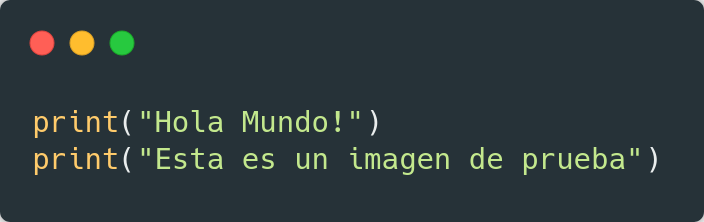
\includegraphics[width=0.5\textwidth]{imagenes/imagenPrueba.png}
		\caption{Descripción de la imagen}
		\label{fig:ejemplo}
	\end{figure}
	
	\section{Desarrollo}
	Aquí va el contenido principal.
	
	\section{Conclusión}
	Aquí va la conclusión del documento.
	
\end{document}
